\documentclass[11pt,a4paper]{article}

\usepackage[utf8]{inputenc}
\usepackage[T1]{fontenc}
\usepackage{lmodern}
\usepackage[spanish,es-noquoting]{babel}
\usepackage[margin=2.3cm]{geometry}
\usepackage{graphicx}
\usepackage{xcolor}
\usepackage{listings}
\usepackage{booktabs}
\usepackage{tabularx}
\usepackage{enumitem}
\usepackage{fancyhdr}
\usepackage[most]{tcolorbox}
\usepackage[hidelinks]{hyperref}

\definecolor{codebg}{HTML}{F6F8FA}
\definecolor{codeframe}{HTML}{D0D7DE}
\definecolor{keyw}{HTML}{0550AE}
\definecolor{strc}{HTML}{0A3069}
\definecolor{comm}{HTML}{6E7781}
\definecolor{okgreen}{HTML}{1A7F37}
\definecolor{badred}{HTML}{CF222E}

\lstdefinelanguage{yaml}{
  keywords={true,false,null},
  morecomment=[l]{\#},
  morestring=[b]', morestring=[b]",
  sensitive=true
}
\lstset{
  basicstyle=\ttfamily\footnotesize,
  backgroundcolor=\color{codebg},
  frame=single, rulecolor=\color{codeframe},
  keywordstyle=\color{keyw}\bfseries,
  stringstyle=\color{strc},
  commentstyle=\color{comm}\itshape,
  breaklines=true, breakatwhitespace=false,
  columns=fullflexible, keepspaces=true,
  showstringspaces=false,
  numbers=left, numberstyle=\tiny\color{comm}, numbersep=6pt,
  xleftmargin=1.6em, framexleftmargin=1.4em,
  literate={á}{{\'a}}1 {é}{{\'e}}1 {í}{{\'i}}1 {ó}{{\'o}}1 {ú}{{\'u}}1
           {ñ}{{\~n}}1 {Á}{{\'A}}1 {É}{{\'E}}1 {Ó}{{\'O}}1 {→}{{$\rightarrow$}}1 {—}{{---}}1
           {─}{{-}}1 {│}{{|}}1 {┌}{{+}}1 {┐}{{+}}1 {└}{{+}}1 {┘}{{+}}1
           {├}{{+}}1 {┤}{{+}}1 {┬}{{+}}1 {┴}{{+}}1 {┼}{{+}}1
}
\lstdefinestyle{plain}{numbers=none, xleftmargin=0pt, framexleftmargin=0pt}

\colorlet{notaback}{blue!3!white}\colorlet{notaframe}{blue!45!black}
\colorlet{avisoback}{red!3!white}\colorlet{avisoframe}{red!55!black}
\newtcolorbox{nota}[1][]{colback=notaback, colframe=notaframe,
  fonttitle=\bfseries, title={#1}, boxrule=0.6pt, arc=1.5mm}
\newtcolorbox{aviso}[1][]{colback=avisoback, colframe=avisoframe,
  fonttitle=\bfseries, title={#1}, boxrule=0.6pt, arc=1.5mm}

\newcommand{\code}[1]{\texttt{#1}}
\newcommand{\repo}{\href{https://github.com/JES0406/mlops-practica-icai}{\code{JES0406/mlops-practica-icai}}}
\newcommand{\run}[1]{\href{https://github.com/JES0406/mlops-practica-icai/actions/runs/#1}{\code{#1}}}
\newcommand{\commit}[1]{\href{https://github.com/JES0406/mlops-practica-icai/commit/#1}{\code{#1}}}

\pagestyle{fancy}
\fancyhf{}
\lhead{\small MLOps --- Kubernetes (GKE) y escaneo de imágenes con Trivy}
\rhead{\small Javier Escobar Serrano}
\cfoot{\thepage}

\title{\textbf{Despliegue en GKE y escaneo de seguridad de imágenes con Trivy}\\[0.4em]
\large Prácticas Unit 4 (Kubernetes) y Unit 5 (Security Images Scanning)}
\author{Javier Escobar Serrano\\
\small Máster en Inteligencia Artificial --- Ingeniería de Modelos 2026-2027}
\date{5 de noviembre de 2026}

\begin{document}
\maketitle
\thispagestyle{empty}

\begin{abstract}
Este informe documenta dos prácticas encadenadas sobre el repositorio \repo{}.
En la primera (Unit 4) se despliega la API de predicción (Flask) y la interfaz
web (Streamlit) del modelo Iris en un clúster de Google Kubernetes Engine (GKE)
desde GitHub Actions, con las imágenes almacenadas en \code{gcr.io}. En la
segunda (Unit 5) se añade un escaneo de vulnerabilidades con Trivy entre la
construcción y la subida de cada imagen, de modo que una vulnerabilidad
\textsc{critical} bloquea el \code{docker push} y, con él, todo el despliegue.
Se muestra el pipeline funcionando, bloqueando una dependencia vulnerable
(\code{pyarrow 13.0.0}, CVE-2023-47248) y volviendo a desplegar tras corregirla.
Todo el trabajo está en la rama \code{p6-k8s-trivy}.
\end{abstract}

\tableofcontents
\newpage

%=====================================================================
\section{Entorno y punto de partida}

\begin{itemize}[nosep]
  \item \textbf{Repositorio:} fork \repo{} de \code{juanviz/mlops-practica-icai},
    con el pipeline DVC + CML (Unit 3) y las imágenes Docker de API y web (Unit 4, Docker).
  \item \textbf{Rama de trabajo:} \code{p6-k8s-trivy}. Cada etapa se subió como un
    \emph{push} independiente para que tenga su propia ejecución en GitHub Actions
    (tabla~\ref{tab:runs}).
  \item \textbf{Google Cloud:} proyecto \code{mlops-icai-a2265f} con facturación
    habilitada; clúster \code{mlops-gke-cluster} en la zona \code{us-central1-a}
    con 2 nodos \code{e2-medium} y GKE 1.36.4.
  \item \textbf{Modelo:} \code{model.pkl} versionado con DVC en DagsHub; el job de
    despliegue lo descarga con \code{dvc pull} antes de construir la imagen de la API.
  \item El cambio de \code{train.py} que pide la nota del enunciado de la Unit 5
    (\code{log\_model(name=..., skops\_trusted\_types=[...])}) ya estaba aplicado.
\end{itemize}

%=====================================================================
\section{Práctica Unit 4: despliegue en GKE}

\subsection{Configuración de Google Cloud}

Se ejecutó con la CLI \code{gcloud} (en una configuración propia, \code{mlops}, para no
tocar otros proyectos):

\begin{lstlisting}[language=bash,style=plain]
gcloud projects create mlops-icai-a2265f --name="MLOps ICAI"
gcloud billing projects link mlops-icai-a2265f --billing-account=<cuenta>
gcloud services enable container.googleapis.com artifactregistry.googleapis.com \
    iam.googleapis.com

# Service account para GitHub Actions
gcloud iam service-accounts create modelos --display-name="MLOps CI deployer"
gcloud projects add-iam-policy-binding mlops-icai-a2265f \
    --member=serviceAccount:modelos@mlops-icai-a2265f.iam.gserviceaccount.com \
    --role=roles/container.admin          # Administrador de Kubernetes Engine
gcloud projects add-iam-policy-binding mlops-icai-a2265f \
    --member=serviceAccount:modelos@mlops-icai-a2265f.iam.gserviceaccount.com \
    --role=roles/artifactregistry.admin   # Administrador de Artifact Registry
gcloud iam service-accounts keys create sa-key.json \
    --iam-account=modelos@mlops-icai-a2265f.iam.gserviceaccount.com

gcloud container clusters create mlops-gke-cluster --zone us-central1-a --num-nodes 2
\end{lstlisting}

Dos pasos adicionales que el enunciado solo menciona en la sección de depuración y que en
un proyecto nuevo hacen falta desde el principio:

\begin{enumerate}[nosep]
  \item \textbf{Repositorio \code{gcr.io} en Artifact Registry.} Google ha retirado
    Container Registry; en proyectos nuevos las rutas \code{gcr.io/<proyecto>/...} solo
    funcionan si existe un repositorio de Artifact Registry con ese nombre:
    \code{gcloud artifacts repositories create gcr.io --repository-format=docker --location=us}.
  \item \textbf{Permiso de lectura para los nodos.} Los nodos descargan las imágenes con
    la \emph{compute service account}; se le concedió
    \code{roles/artifactregistry.reader} para evitar errores \code{ImagePullBackOff}.
\end{enumerate}

\subsection{Variables y secretos en GitHub}

Con \code{gh} se definieron en \emph{Settings $\rightarrow$ Secrets and variables
$\rightarrow$ Actions}:

\begin{center}
\begin{tabular}{lll}
\toprule
Nombre & Tipo & Valor \\
\midrule
\code{GCP\_PROJECT\_ID} & variable & \code{mlops-icai-a2265f} \\
\code{GKE\_CLUSTER}     & variable & \code{mlops-gke-cluster} \\
\code{GKE\_ZONE}        & variable & \code{us-central1-a} \\
\code{GCP\_SA\_KEY}     & secret   & JSON de la clave de \code{modelos@...} \\
\bottomrule
\end{tabular}
\end{center}

La clave JSON nunca se ha guardado en el repositorio; GitHub la enmascara en los logs
(se comprobó que ninguno de los logs guardados contiene \code{private\_key}).

\subsection{Manifiestos de Kubernetes}

Primero se desplegó solo la API (\code{deployment.yaml} + \code{service.yaml} de tipo
\code{LoadBalancer}, commit \commit{4902306}). Después, siguiendo la sección 4 del
enunciado, se renombraron a \code{api-*.yaml}, el Service de la API pasó a
\code{ClusterIP} en el puerto 5000 (solo accesible dentro del clúster) y se añadieron
el Deployment y el Service públicos de la web (commit \commit{bd9a172}).

\lstinputlisting[language=yaml,title={\code{api-deployment.yaml}}]{../api-deployment.yaml}
\lstinputlisting[language=yaml,title={\code{api-service.yaml}}]{../api-service.yaml}
\lstinputlisting[language=yaml,title={\code{web-deployment.yaml}}]{../web-deployment.yaml}
\lstinputlisting[language=yaml,title={\code{web-service.yaml}}]{../web-service.yaml}

La web localiza la API por DNS interno de Kubernetes
(\code{http://mlops-api-service:5000/predict}), que \code{app\_web.py} lee de la
variable de entorno \code{API\_URL}.

\subsection{Job \code{deploy-to-gke}}

Se añadió al workflow \code{.github/workflows/cml.yaml} un segundo job que depende de
\code{train-and-report}. El listado~\ref{lst:job} muestra su versión final (ya con los
pasos de Trivy de la Unit 5 y las comprobaciones finales). Respecto al enunciado:

\begin{itemize}[nosep]
  \item \textbf{\emph{Fix} de CML:} se sustituyó \code{iterative/setup-cml} por
    \code{npm install -g @dvcorg/cml}, como indica el enunciado.
  \item \textbf{\code{dvc pull}:} se reutiliza la autenticación \code{basic} con usuario
    y token de DagsHub que ya usaba el job de entrenamiento.
  \item \textbf{Solo en \code{push}:} el workflow se dispara con \code{push} y con
    \code{pull\_request}; el despliegue se limita a \code{push} para no desplegar dos
    veces el mismo commit.
  \item \textbf{\code{kubectl rollout restart}:} las imágenes usan siempre la etiqueta
    \code{latest}; como el spec del Deployment no cambia, \code{kubectl apply} no
    reinicia los pods. El reinicio fuerza a descargar la imagen recién subida, y
    \code{rollout status} hace que el job falle si los pods no arrancan.
  \item \textbf{Acciones fijadas a commit:} \code{google-github-actions/auth} y
    \code{setup-gcloud} se referencian por SHA (commit \commit{99bff29}) en vez de por
    etiqueta, igual que las acciones de \code{iterative} en la práctica anterior. Estas
    acciones manejan la clave de la service account.
\end{itemize}

\lstinputlisting[language=yaml,firstline=97,caption={Job \code{deploy-to-gke} (versión final)},label={lst:job}]{../.github/workflows/cml.yaml}

\subsection{Verificación}

\paragraph{API (solo API desplegada, ejecución \run{41996993196}).}
El job aplicó los manifiestos y el \emph{rollout} terminó correctamente. La prueba del
enunciado contra la IP pública del LoadBalancer de la API devolvió la clase correcta
(\emph{Setosa}):

\begin{lstlisting}[language=bash,style=plain]
$ curl -X POST -H "Content-Type: application/json" \
       -d '{"features": [5.1, 3.5, 1.4, 0.2]}' http://136.64.56.38/predict
{"prediction":0}
\end{lstlisting}

\paragraph{API + web (ejecución \run{42004275345}).}
Salida de \code{kubectl get svc} al final del job:

\begin{lstlisting}[style=plain]
NAME                TYPE           CLUSTER-IP       EXTERNAL-IP   PORT(S)        AGE
kubernetes          ClusterIP      34.118.224.1     <none>        443/TCP        62m
mlops-api-service   ClusterIP      34.118.229.106   <none>        5000/TCP       7m22s
mlops-web-service   LoadBalancer   34.118.227.138   <pending>     80:30107/TCP   18s
\end{lstlisting}

La API dejó de ser accesible desde fuera (la antigua IP \code{136.64.56.38} ya no
responde) y la web quedó publicada en \url{http://35.253.244.201}.

\paragraph{Comprobación web.}
La IP pública del Service \code{mlops-web-service} se obtuvo con
\code{gcloud compute forwarding-rules list} (equivale a la columna \code{EXTERNAL-IP} de
\code{kubectl get svc} o a la consola de GKE). La figura~\ref{fig:web} muestra la
interfaz servida desde GKE: la web llama a la API por el Service interno y muestra la
especie predicha.

\begin{figure}[h]
\centering
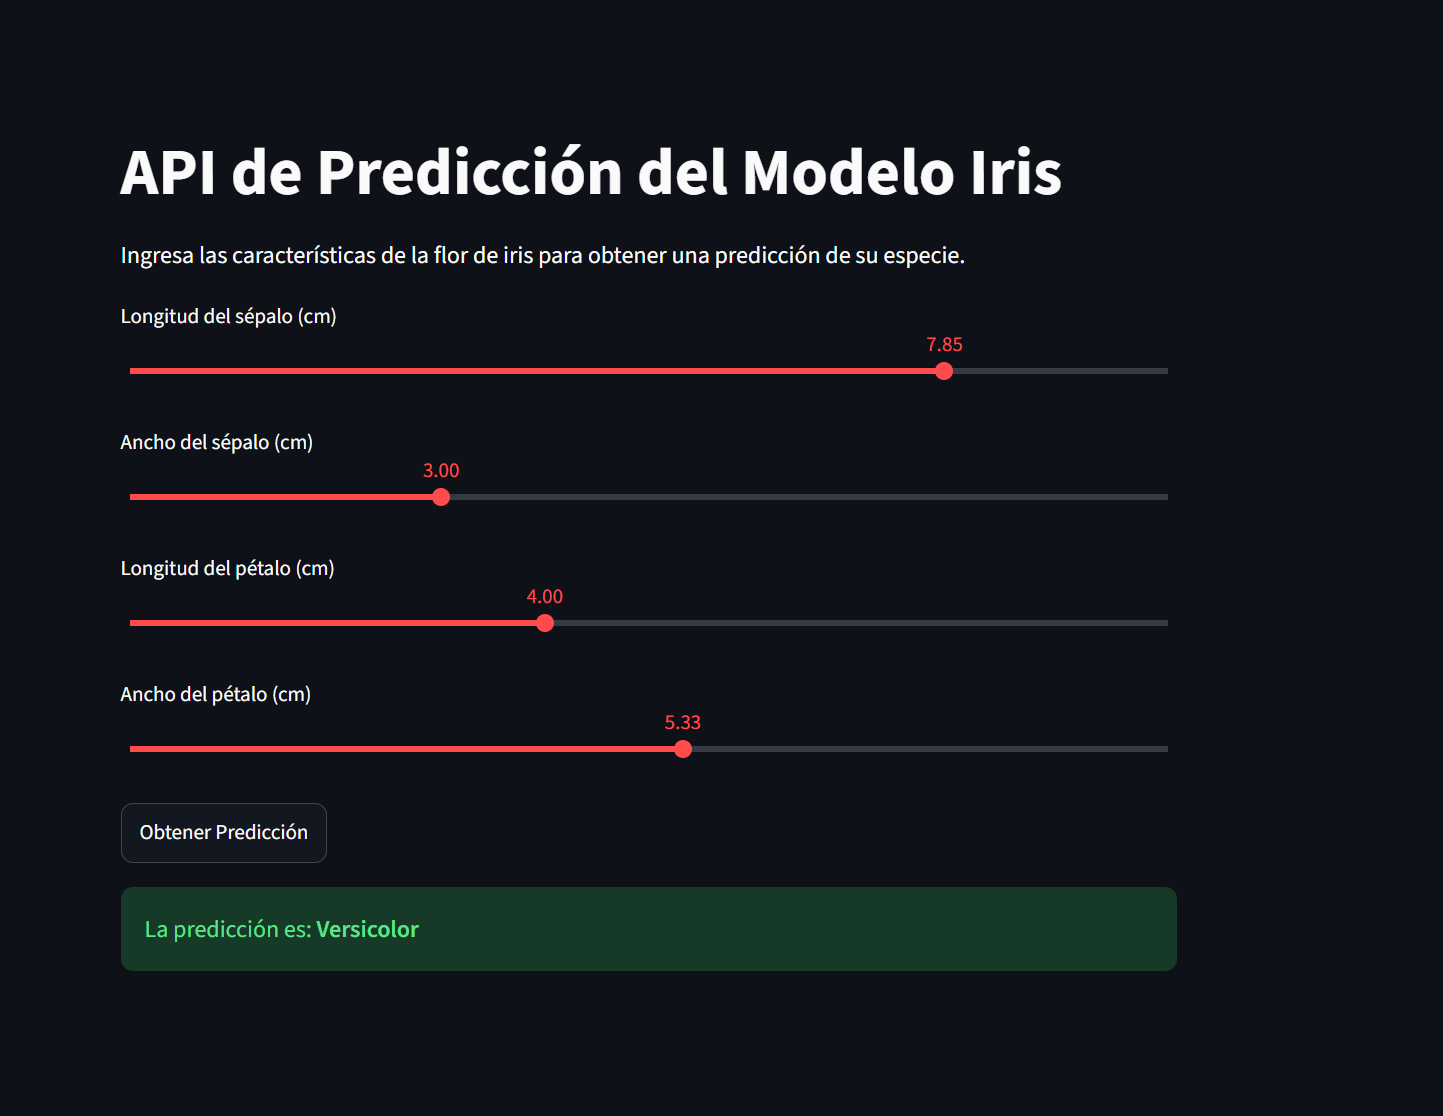
\includegraphics[width=0.78\textwidth]{figures/web-gke-prediccion.png}
\caption{Streamlit desplegado en GKE (\url{http://35.253.244.201}) devolviendo una
predicción a través de la API interna.}
\label{fig:web}
\end{figure}

\paragraph{Prueba automática tras el despliegue.}\label{sec:smoke}
Además se añadió al final del job un paso \emph{Smoke test} (commits \commit{d097049} y
\commit{422bbe2}) que falla el pipeline si el despliegue no funciona de extremo a extremo:
\begin{enumerate}[nosep]
  \item ejecuta dentro del pod web (\code{kubectl exec}) una petición a
    \code{\$API\_URL}, es decir, el mismo camino web $\rightarrow$ API que usa Streamlit;
  \item espera a que el LoadBalancer de la web tenga IP y comprueba que responde HTTP 200;
  \item hace el \emph{handshake} del websocket de Streamlit (\code{/\_stcore/stream}) y
    exige \code{101 Switching Protocols}, ya que sin él la página no llega a pintarse.
\end{enumerate}

Salida del paso en la ejecución final \run{42007215102}:

\begin{lstlisting}[style=plain]
200 ***"prediction":0***          # web -> API dentro del clúster
Web: http://35.253.244.201
HTTP 200
WebSocket: HTTP/1.1 101 Switching Protocols
\end{lstlisting}

Las llaves de \code{\{"prediction":0\}} aparecen como \code{***} porque GitHub enmascara
cada línea del secreto \code{GCP\_SA\_KEY}, y el JSON de la clave tiene líneas que son
solo \code{\{} y \code{\}}.

%=====================================================================
\section{Práctica Unit 5: escaneo de imágenes con Trivy}

\subsection{Puerta de seguridad en el pipeline}

En el job \code{deploy-to-gke} los pasos ``construir y subir'' de cada imagen se
sustituyeron por tres pasos (commit \commit{ce7b369}):

\begin{enumerate}[nosep]
  \item \textbf{Build}: \code{docker build} de \code{gcr.io/<proyecto>/mlops-api:latest}
    (o \code{mlops-web}) y se exporta el nombre en \code{\$GITHUB\_ENV}.
  \item \textbf{Trivy}: \code{aquasecurity/trivy-action} sobre la imagen local con
    \code{severity: CRITICAL} y \code{exit-code: '1'}.
  \item \textbf{Push}: \code{docker push}, que solo se ejecuta si el escaneo ha pasado.
\end{enumerate}

Si Trivy encuentra una vulnerabilidad \textsc{critical}, el paso falla, GitHub Actions
salta todos los pasos siguientes (\code{push} y \code{Deploy to GKE}) y en el clúster
sigue corriendo la última versión buena.

\begin{aviso}[Desviación: \code{trivy-action} fijada a un commit, no a \code{@master}]
El enunciado usa \code{aquasecurity/trivy-action@master}. En marzo de 2026 el propio
ecosistema de Trivy sufrió un ataque de cadena de suministro (aviso
\href{https://github.com/aquasecurity/trivy/security/advisories/GHSA-69fq-xp46-6x23}{GHSA-69fq-xp46-6x23}):
los atacantes reescribieron 76 de las 77 etiquetas de \code{trivy-action} para que
ejecutaran un ladrón de credenciales que vuelca la memoria del runner, y publicaron
imágenes de Trivy maliciosas (v0.69.4--v0.69.6). En este workflow eso significaría
filtrar \code{GCP\_SA\_KEY}, con permisos de administrador sobre GKE y Artifact Registry.

Por eso la acción se fija al commit de la release inmutable v0.36.0
(\code{ed142fd0673e97e23eac54620cfb913e5ce36c25}) y se indica explícitamente la versión
de Trivy (\code{version: 'v0.76.1'}). Para los escaneos locales se usa la imagen
\code{aquasec/trivy:0.76.1} referenciada por \emph{digest}.
\end{aviso}

\subsection{Etapa A: escaneo con las dependencias actuales}

El \code{requirements.txt} del repositorio no fija \code{mlflow} (se instala la última,
3.18.0), así que no reproduce la tabla del enunciado (\code{mlflow 2.8.0},
\code{pyarrow 13.0.0}, \dots). En la ejecución \run{42005391746} Trivy no encontró
ninguna vulnerabilidad \textsc{critical} en ninguna de las dos imágenes, las imágenes se
subieron y se desplegaron:

\begin{lstlisting}[style=plain]
gcr.io/mlops-icai-a2265f/mlops-api:latest (debian 13.7)   debian   0
latest: digest: sha256:3433f1089fd5b7616526f9472e2f53f438feafc54b972050ef10a82700b507d9
gcr.io/mlops-icai-a2265f/mlops-web:latest (debian 13.7)   debian   0
latest: digest: sha256:989caf0677b15716a61ac8f6a2424034cda5360fd186ae78473989192b642a09
\end{lstlisting}

\subsection{Etapa B: dependencias vulnerables (la puerta bloquea)}

Para comprobar que la puerta bloquea de verdad, se fijaron a propósito las versiones
vulnerables de la tabla del enunciado (commit \commit{858489b}):

\begin{lstlisting}[style=plain]
pyarrow==13.0.0
gunicorn==21.2.0
setuptools==65.5.1
\end{lstlisting}

\begin{nota}[Por qué no se fijó \code{mlflow==2.8.0}]
\code{train.py} usa la API de mlflow 3 (\code{log\_model(model, name=...,
skops\_trusted\_types=[...])}), que no existe en 2.8.0, y \code{requirements.txt} es
dependencia de la etapa \code{train} de DVC: el job \code{train-and-report} habría fallado
antes de llegar al escaneo. Con \code{pyarrow 13.0.0} ya hay una vulnerabilidad
\textsc{critical} y pip resuelve sin conflictos (\code{mlflow 3.18.0} acepta esa versión).
\end{nota}

En la ejecución \run{42006388026} el escaneo de la imagen de la API falló y GitHub Actions
saltó todos los pasos posteriores; no se subió ninguna imagen y en GKE siguió la versión
de la etapa A:

\begin{lstlisting}[style=plain]
Total: 1 (CRITICAL: 1)
| Library | Vulnerability  | Severity | Status | Installed | Fixed  | Title
| pyarrow | CVE-2023-47248 | CRITICAL | fixed  | 13.0.0    | 14.0.1 | PyArrow: Arbitrary
                                                                    code execution when
                                                                    loading a malicious
                                                                    data file
##[error]Process completed with exit code 1.
\end{lstlisting}

\begin{center}
\begin{tabular}{ll}
\toprule
Paso del job \code{deploy-to-gke} & Resultado \\
\midrule
Build API Docker Image & \textcolor{okgreen}{success} \\
Trivy Scan for API Image & \textcolor{badred}{failure} \\
Push API Docker Image & skipped \\
Build / Trivy / Push Web Docker Image & skipped \\
Deploy to GKE & skipped \\
\bottomrule
\end{tabular}
\end{center}

CVE-2023-47248 permite ejecutar código arbitrario al leer un fichero IPC/Parquet
malicioso, porque \code{pyarrow} deserializaba con \code{pickle} el tipo de extensión
\code{arrow.py\_extension\_type}.

\subsection{Etapa C: corrección de \code{requirements.txt}}

Se sustituyeron las versiones vulnerables por las mínimas corregidas de la tabla del
enunciado (commit \commit{0468cc0}):

\begin{lstlisting}[style=plain]
pyarrow>=14.0.1      # CVE-2023-47248 (CRITICAL) en 13.0.0
gunicorn>=22.0.0     # vulnerabilidades HIGH en 21.2.0
setuptools>=70.0.0   # vulnerabilidades HIGH en 65.5.1
\end{lstlisting}

pip instaló \code{pyarrow 26.0.1}, \code{gunicorn 26.2.0} y \code{setuptools 79.0.1}
(\code{mlflow} sigue en 3.18.0). En la ejecución \run{42007215102} los dos escaneos
pasaron, las imágenes se subieron y se desplegaron, y la prueba automática final
(sección~\ref{sec:smoke}) fue correcta:

\begin{lstlisting}[style=plain]
gcr.io/mlops-icai-a2265f/mlops-api:latest (debian 13.7)   debian   0
latest: digest: sha256:af6d16aae23cb83f7d48af5f339117f6dbbb77fed475db00a59f7aa74983aae0
gcr.io/mlops-icai-a2265f/mlops-web:latest (debian 13.7)   debian   0
latest: digest: sha256:864f7c65e4e2dee8b796dc99bfedb58b65c94a8aad78c2eb8fc36a0f55380a0f
deployment "mlops-api-deployment" successfully rolled out
deployment "mlops-web-deployment" successfully rolled out
\end{lstlisting}

\subsection{Escaneo local (\textsc{critical} y \textsc{high})}

El enunciado propone ejecutar Trivy en local con \code{--severity CRITICAL,HIGH}. En
Windows/WSL se usó el contenedor oficial; al comando del enunciado le falta montar el
socket de Docker, sin el cual Trivy no ve las imágenes locales:

\begin{lstlisting}[language=bash,style=plain]
docker run --rm -v /var/run/docker.sock:/var/run/docker.sock \
  -v $HOME/trivy-cache:/root/.cache/ \
  aquasec/trivy:0.76.1@sha256:790fd66d1697395d8693d1acaa1ea702406a20f109b6fc7bac8db623eca6c06c \
  image --severity CRITICAL,HIGH --exit-code 1 mlops-web:latest
\end{lstlisting}

\begin{center}
\begin{tabular}{lcccc}
\toprule
Imagen & Dependencias & \textsc{critical} & \textsc{high} (Debian) & \textsc{high} (Python) \\
\midrule
\code{mlops-api} & actuales & 0 & 48 & 2 \\
\code{mlops-web} & actuales & 0 & 48 & 2 \\
\code{mlops-web} & vulnerables (etapa B) & \textcolor{badred}{1} & --- & --- \\
\code{mlops-web} & corregidas (etapa C) & \textcolor{okgreen}{0} & 48 & 2 \\
\bottomrule
\end{tabular}
\end{center}

Las 48 vulnerabilidades \textsc{high} restantes son paquetes del sistema de la imagen base
\code{python:3.11-slim} (Debian 13.7) y las 2 de Python están en librerías que
\code{setuptools} lleva dentro (\code{jaraco.context}, \code{wheel}). No dependen del
\code{requirements.txt}; para eliminarlas habría que actualizar la imagen base o
instalar parches con \code{apt-get upgrade} en el Dockerfile. Con el umbral del
pipeline (\textsc{critical}) no bloquean el despliegue.

%=====================================================================
\section{Problemas encontrados}

\begin{description}[style=nextline]
  \item[GitHub Actions bloqueado por facturación]
    Los primeros intentos fallaban antes de empezar con
    \emph{``The job was not started because your account is locked due to a billing
    issue''}. La cuenta tenía un presupuesto de Actions de 0\,\$ con ``stop usage'', y
    un consumo mínimo (<\,0{,}01\,\$, cubierto por el uso incluido) bastaba para marcarlo
    al 100\,\%. Se resolvió desde la configuración de facturación de GitHub.
  \item[La web se queda cargando desde la red de la universidad]
    La página HTML y el JavaScript de Streamlit cargaban (HTTP 200), pero la interfaz no
    se pintaba. Streamlit necesita abrir un websocket en \code{/\_stcore/stream}; desde la
    red local esa conexión se cortaba siempre (\emph{connection reset}). La misma imagen en
    local respondía \code{101 Switching Protocols}, y servidores de eco websocket públicos
    en el puerto 80 también eran cortados desde esa red, así que la causa es un filtro de
    la red (websockets sin TLS en el puerto 80), no el despliegue. Para comprobarlo desde
    fuera se añadió al pipeline una prueba que hace el \emph{handshake} desde el runner de
    GitHub (sección~\ref{sec:smoke}).
  \item[\code{kubectl} local sin \code{gke-gcloud-auth-plugin}]
    No fue necesario: todo el despliegue lo hace el pipeline y las IPs públicas se
    consultaron con \code{gcloud compute forwarding-rules list}.
\end{description}

%=====================================================================
\section{Resumen de ejecuciones}

\begin{table}[h]
\centering
\begin{tabularx}{\textwidth}{l l X c}
\toprule
Ejecución & Commit & Contenido & Resultado \\
\midrule
\run{41996993196} & \commit{99bff29} & Solo API en GKE (LoadBalancer) & \textcolor{okgreen}{OK} \\
\run{42004275345} & \commit{bd9a172} & API (ClusterIP) + web (LoadBalancer) & \textcolor{okgreen}{OK} \\
\run{42005391746} & \commit{ce7b369} & Puerta Trivy, dependencias actuales & \textcolor{okgreen}{OK} \\
\run{42006388026} & \commit{858489b} & Dependencias vulnerables (\code{pyarrow 13.0.0}) & \textcolor{badred}{Bloqueado} \\
\run{42007215102} & \commit{422bbe2} & Dependencias corregidas + prueba automática & \textcolor{okgreen}{OK} \\
\bottomrule
\end{tabularx}
\caption{Ejecuciones de GitHub Actions en la rama \code{p6-k8s-trivy}.}
\label{tab:runs}
\end{table}

%=====================================================================
\section{Costes y limpieza}

El clúster (2 nodos \code{e2-medium}) y los dos balanceadores cuestan del orden de
3--5\,\$ al día. Tras la corrección se elimina el clúster con
\code{gcloud container clusters delete mlops-gke-cluster --zone us-central1-a}; el
proyecto, la service account y las imágenes en \code{gcr.io} se conservan.

\section{Conclusiones}

\begin{itemize}[nosep]
  \item Cada \emph{push} a la rama entrena el modelo, construye las dos imágenes, las
    escanea y, solo si están limpias, las sube a \code{gcr.io} y las despliega en GKE.
  \item La API queda interna (\code{ClusterIP}) y solo la web es pública, lo que reduce
    la superficie expuesta.
  \item La puerta de Trivy cumple su función: una dependencia con una vulnerabilidad
    crítica de ejecución de código (\code{pyarrow 13.0.0}) no llega al registro ni al
    clúster.
  \item La propia herramienta de seguridad es parte de la cadena de suministro: fijar
    acciones y herramientas a commits/digests inmutables es tan importante como escanear.
    Como mejora, la clave JSON de larga duración podría sustituirse por
    \emph{Workload Identity Federation}, de modo que no haya ningún secreto que robar.
\end{itemize}

\end{document}
